
\documentclass[preprint,10pt,5p,twocolumn]{elsarticle}
%\documentclass[preprint,authoryear,10pt,5p,twocolumn]{elsarticle}

\usepackage{amsmath}
\usepackage{graphicx}
\usepackage{subfigure}

%% for the old format  ( remove this and the abstract and the bibgraphy style. )
%\documentclass{article}
%\usepackage{spconf}
%\usepackage{amsmath}
%\usepackage[dvips,pdftex]{graphicx}
%\usepackage{named}
%\usepackage[dvips,pdftex]{hyperref}

%\title{Sketch Recognition using Particle Swarm Optimizations}
%\twoauthors
%  {Maha El Meseery\sthanks{Corresponding Author}, Mahmoud Fakhr El Din\sthanks{Associate Professor}, Samia Mashali\sthanks{Professor}}
%	{Signals Processing Group \\ Computers and Systems Department \\
%  Electronic Research Institute\\Cairo, Egypt\\
%	melmeseery@eri.sci.eg, mafakhr@mcit.gov.eg,\\ samia@eri.sci.eg}
%  {Magda Fayek\sthanks{Associate Professor}, Nevin Darwish\sthanks{Professor}}
%	{Computer Engineering Department\\
%	Faculty of Engineering \\Cairo University\\Cairo, Egypt\\
%	magdafayek@gmail.com,ndarwish@ieee.org}
%\maketitle

\begin{document}
\begin{frontmatter}
\title{Sketch Recognition using Particle Swarm Optimizations}

%% use optional labels to link authors explicitly to addresses:
%% \author[label1,label2]{<author name>}
%% \address[label1]{<address>}
%% \address[label2]{<address>}

\author[ERI]{Maha El Meseery\footnote{Crossponding author}}
\author[ERI]{Mahmoud Fakhr El Din}
\author[ERI]{Samia Mashali}
\author[FAC]{Magda Fayek}
\author[FAC]{Nevin Darwish}
\address[ERI]{Signals Processing Group, Computers and Systems Department, 
  Electronic Research Institute, Cairo, Egypt\\melmeseery@eri.sci.eg, mafakhr@mcit.gov.eg, samia@eri.sci.eg}
\address[FAC]{Computer Engineering Department,
	Faculty of Engineering,Cairo University, Cairo, Egypt\\
	magdafayek@gmail.com,ndarwish@ieee.org}
\begin{abstract}
%%This study 
Sketches and drawings are widely used as simple methods of expressing thought and designs. The goal of this paper is developing a sketch recognition system that facilitates using sketches in computer systems. The system uses Particle Swarm Optimization (PSO) algorithm to optimally segment the strokes the user draws into meaningful geometric primitives.  These geometric primitives are grouped to form symbols which are further identified using a Support Vector Machines (SVM) classifier. Two versions of PSO segmentation algorithms were implemented. Experiments were conducted on three different dataset, simple presentation (Hs-DS), Electrical Design (EL-DS) and Logic Design (LD-DS) symbols. Results show that both PSO algorithms produce better segmentation than most current systems. This segmentation improvement contributed in getting more accurate recognition results on all the datasets tested. The results prove that the system is effective specially in datasets with low diversity in shapes, i.e., shapes are very simillar, as in Logic Design dataset (LD-DS). %The results prove the effectiveness of the proposed system on various dataset, especially datasets with low shape diversity as in Logic Design dataset (LD-DS).% effectiveness of the proposed system on various dataset, especially datasets with low shape diversity as in Logic Design dataset (LD-DS). %Result show that the system is especially effictive on dataset with % sketch are divided  Users draw symbols and sketchs using a set of pen strokes. 
%%Sketch recognition is defined as the process of identifying symbols that users draw using single or multiple strokes. Usually, users draw strokes using pens. The sketch recognition system immediately interprets their strokes as objects that can be easily manipulated. This paper uses Particle Swarm Optimization (PSO) to divide the strokes the user draws into meaningful geometric primitives. These geometric primitives are grouped to formulate symbols which are further identified. The results show that using PSO improves segmentation results which guide the symbol recognition phase. As for recognition we use Support Vector Machines (SVM) classifier which further improves the final recognition accuracy.  

\end{abstract}

\begin{keyword}
%% keywords here, in the form: keyword \sep keyword
Symbol Recognition, Particle Swarm Optimization, Sketch Recognition, Geometerical Features, Polygon approximation
%% PACS codes here, in the form: \PACS code \sep code

%% MSC codes here, in the form: \MSC code \sep code
%% or \MSC[2008] code \sep code (2000 is the default)

\end{keyword}

\end{frontmatter}



%\begin{abstract}
%%This study 
%Sketches and drawings are widely used as a simple method of expressing thought and designs. The goal of this paper is developing a sketch recognition system that facilitates using sketches in computer systems. The system uses Particle Swarm Optimization (PSO) algorithm to optimally segment the strokes the user draws into meaningful geometric primitives.  These geometric primitives are grouped to formulate symbols which are further identified using a Support Vector Machines (SVM) classifier. Two different segmentation algorithms were evaluated and results show that both algorithms improve the final recognition results. Experiments were conducted on three different dataset, simple presentation (Hs-DB), Electrical Design (EL-DB) and Logic Design (LD-DB) symbols. Results show that the effectiveness of the proposed system on various dataset especially on datasets with low shape diversity as in Logic Design dataset (LD-DS).  % sketch are divided  Users draw symbols and sketchs using a set of pen strokes. 
%%Sketch recognition is defined as the process of identifying symbols that users draw using single or multiple %strokes. Usually, users draw strokes using pens. The sketch recognition system immediately interprets their %strokes as objects that can be easily manipulated. This paper uses Particle Swarm Optimization (PSO) to divide %the strokes the user draws into meaningful geometric primitives. These geometric primitives are grouped to %formulate symbols which are further identified. The results show that using PSO improves segmentation results %which guide the symbol recognition phase. As for recognition we use Support Vector Machines (SVM) classifier %which further improves the final recognition accuracy.  
%\end{abstract}

\section{Introduction}

Computer research nowadays aims at facilitating computer human interaction in every way. Pen-based interfaces give the user a pencil-paper like feeling that enhances interaction more than the current used keyboard-mouse computer interfaces. However, using sketches as input to a computer system requires the system to understand the drawn sketches. In a truly freely sketch system this is not a trivial problem due to the sloppy and messy  way in which users draw sketches. Sketches here stand for any hand drawing the user draws using digital stylus or similar device. Normally, sketches are composed of a set of strokes. The time between pen-up and pen-down events identifies each stroke. The strokes are mainly the path of points, which the user draws between the pen-down and pen-up events while using the stylus or similar device. 

Sketch recognition can be applied either using  Pattern Recognition (PR) based method or Artifical Intelligance (AI) based method. In AI based methods, Symbols are represented using hierarchical levels of simpler geometric shapes or primitives and spatial relations between them. Systems that employ such representation must first pre-process. strokes to break them into geometric primitives. Recognition can then is treated as an AI problem which can be solved using methods like sub graph matching, bayes belief network, and constrain statisfaction. A Hierarchical shape descriptions was widely used in sketch systems \cite{HierarchicalParsing7,SketchRead2007}.  %Ladder30,AlvaradoFreedom42


Recognition based on AI methods as applied in \cite{SketchRead2007} has the principle problem of computational complexity of the matching between shape description and geometric primitives produced in the segmentation process. Natural sketch are difficult to be segmented and grouped to create reliable fragment of geometric primitives. This is partially due to the increase of noise and other phenomena such as overlapped, over traced strokes and sharing of strokes between different symbols. Since these systems are dependable on the segmentation results, they either perform recognition using undependable segmentation results or consider different ways to segment the input sketch. This is because they assume that each stroke plays a role in the structure of the shape. 
%The role of which each stroke plays in the structure of the sketched symbol is used to determine shapes in stroke based methods.  
%Gestures are pen strokes drawn by the user that can immediately recognized by the system.
%role of which each stroke plays in the structure of the sketched symbol is used to determine shapes 
%. discribing the role  how user draws individal storkes  properties that discribe how users draw individual strokes in drawing the symbol.  to . The identification of individual stroke is used to determine  The symbols are recognized by identifing the individual strokes.
In PR based methods, systems compute properties that discribe symbols then use a classification method to recognize symbols. The properties used can either be based on gesture properties, global shape properties or image based properties. Gesture properties are set of features that represent how the user draws a symbol not how it looks like (e.g., identify a regtangle when a user draws a L corner). In gesture properties approcah, systems identify symbols by using gesutre properties of some of its  underlying strokes. System that uses gestures properties assume that users draw symbols in specific order and style \cite{gestureexample12,aideddesgin22}. In global shape properties approach, systems investigate general shape properties and its underlying strokes. Using shape properties (e.g., ratio of the area of convex hull to the area of shape) relaxes the assumption and the role of each stroke in the symbol but it does not truly represent the appearance or fine details of the symbol \cite{DiagramOfflineConvexHull,Cali63}. Unlike shape properties based methods, image based methods disregard individual strokes and focus on the overall appearance of shapes. These system convertes the shapes into image and extracte image based features (e.g. local gradient feature)\cite{Oltmans07,imagetrainable48}. In \cite{imagetrainable48}, they used four different distance measures to to match user symbol with the prototype database. The prototype of a shape is represented as an image of the symbol that is normalized and scaled.  However, the problem is that the shape prototype must represent all transformation and variation the input shape can have.   %Image based methods are used in \cite{Oltmans07,imagetrainable48} where they computed a code book of 1000 features to recognize symbols. 

Methods based on gesture and global shape properties produce systems that are dependent on assumptions about how strokes can be grouped. These systems assume that users will finish drawing a shape before moving to the next one \cite{Cali63,geometrydomain49}. This assumption allows the system to temporally group strokes and then recognizes them based on their strokes or global shape properties. Alvarado \cite{AlvaradoDigital} argued that this assumption does not hold in natural sketches. 


In this paper, we choose to implement a hybrid method between shape property, guesture and hierarchical (AI method) based approaches. Our method attempts to avoid many of the problems faced by approaches based on individual guestures or global shape properties while trying to gain the additional information that the stroke based system uses. Firstly, the system uses particle swarm optimization (PSO) to optimally segment user's strokes. Users can draw symbols using any number of strokes in any order they like. The system segments each stroke using two different PSO algorithms. The first segmentation algorithm is based on dividing the digital curve into polygons\cite{PolygonApproximationPSO}. Our algorithm enhances its performance by adding curvature and other local information while segmenting strokes to achieve better results. To handle complex strokes, our system uses a second segmentation PSO algorithm to segment strokes into a set of lines and circular arcs. After segmentation, a feature vector composed of different statistical, geometrical and composite features is deduced. The final classification step uses a SVM classifier to classify symbols into one of the previously trained classes based on the features vector computed.


 %In general, the  appearance based methods use image processing techniques to recognize sketches that the users draw. 
%Sketch recognition can be based on: strokes, global shape properties, and appearance \cite{Oltmans07}. The role of which each stroke plays in the structure of the sketched symbol is used to determine shapes in stroke based methods. Most stroke based systems either represent symbols as gestures or as a  hierarchical shape. Gestures are pen strokes drawn by the user that can immediately recognized by the system. A Hierarchical shape descriptions was widely used in sketch systems \cite{HierarchicalParsing7,Ladder30,AlvaradoFreedom42,SketchRead2007}. Symbols are represented using hierarchical levels of simpler geometric shapes or primitives and spatial relations between them. Systems that employ such representation must first pre-process strokes to break them into geometric primitives. Recognition can hen be treated as sub graph matching problem.   

 %In global shape properties approach, systems investigate general shape properties and its underlying strokes. Using shape properties (i.e. ratio of area of convex hull to area of shape) relaxes the assumption and role of each stroke in the symbol but it does not truly represent the appearance of the symbol\cite{DiagramOfflineConvexHull}. Unlike appearance based methods where individual strokes are disregarded and they focus on the overall appearance of shapes. In general, the  appearance based methods use image processing techniques to recognize sketches that the users draw. 
  
 %Methods based on gesture and global shape properties produce systems that are dependent on assumptions about how strokes can be grouped. These systems assume that users will finish drawing a shape before moving to the next one \cite{Cali63,geometrydomain49}. This let them to temporally group strokes and then recognizes them based on their strokes or global shape properties. \cite{AlvaradoDigital} argued that this assumption does not hold in natural sketches.
 
 %Recognition based on strokes using hierarchical shape description is applied in \cite{SketchRead2007}. The principle problem in these systems is the computational complexity of the matching between shape description and geometric primitives produced in the segmentation process. Natural sketch are difficult to segment and group to create reliable fragment of geometric primitives. This is partially due to the increase of noise and other phenomena such as overlapped, over traced strokes and sharing of strokes between different symbols. Since these systems are dependable on the segmentation results, they either perform recognition using undependable segmentation results or consider different ways to segment the input sketch. 
 
%In this paper we choose to implement a hybrid method between shape property and stroke based approaches. Our method tries to avoid many of the problems faced by approaches based on individual strokes or global shape properties while trying to gain the additional information that the stroke based system use. Firstly, the system uses particle swarm optimization (PSO) to optimally segment user's strokes. Users can draw symbols using any number of strokes in any order they like. The system segments each stroke using two different PSO algorithms. The first segmentation algorithm is based on dividing the digital curve into polygons\cite{PolygonApproximationPSO}. Our algorithm enhances its performance by adding curvature and other local information while segmenting strokes to achieve better results. To handle complex strokes, our system uses a second segmentation PSO algorithm to segment strokes into a set of lines and circular arcs. After segmentation, a feature vector composed of different statistical, geometrical and composite features is deduced. The final classification step uses a SVM classifier to classify symbols into one of the previously trained classes based on the features vector computed.

 %The preprocessing phase captures user input stroke points and collects basic information about the stroke. In the segmentation phase, the strokes are divided into a set of simple geometrical primitives or segments. In the third phase, sketch recognition, strokes and segments are clustered to formulate symbols that can be recognized by a classifier. 

%This paper introduces a new sketch recognition system, which uses  % uses the computed feature vector to classify the segments into one of the previously trained classes.
%Sections \ref{Prepross}, \ref{seg} and \ref{sec:Recognition} provide details on preprocessing, segmentation and recognition process respectively.
 The remaining of the paper is as follows; the literature review on stroke segmentation is presented in Section \ref{sec:review}. Section \ref{sec:ParticleSwarmAlgorithm} introduces Particle Swarm Optimization. Section \ref{Sysdisc} describes the proposed system in details. Section \ref{sec:Experiments} describes the experiments that were preformed. Finally, the conclusion and future work is presented in Section \ref{ConclusionandFutureWork}.  

\section{Literature Review}
\label{sec:review}

Yu \cite{meanshift10} introduced a \textit{feature area} for each primitive and then computed the segmentation error for different types of primitives based on the computed \textit{feature area}. His system achieved good accuracy in simple shapes (square, ellipse,...etc) but did not perform well in complex shapes. A hybrid algorithm was introduced in \cite{earlyprocess} where different sets of segments are generated based on both curvature and speed dominant points, followed by choosing a segmentation with the least error from a generated hybrid set. However, this system is limited to recognizing only specific simple geometric shapes with a set of low level recognizers. Each low level recognizer is designed to recognize only one geometric shape using spatial and geometric information extracted from input stroke. 

A genetic algorithm was used by \cite{CruveDivisionSwarm} to optimally divide digital curves into lines and curves. Chen et al. \cite{CruveDivisionSwarm} uses digital curves scanned from paper as input to the system. However, they did not take the advantage of the curvature or local geometric properties of the digital curve. Yin \cite{PolygonApproximationPSO} used PSO to convert digital curves into polygons. Our system adopts  Yin \cite{PolygonApproximationPSO} method and tries to improve it by adding curvature and other local information while segmenting strokes to achieve better segmentations. The next section presents the general particle swarm algorithm which is used in this system.

 % are presented in section \ref{subsubsec:Discreteparticleswarmalgorithm}

\section{Discrete Particle Swarm Optimization}
\label{sec:ParticleSwarmAlgorithm}
%\section{Particle Swarm Algorithm}
%\label{PSO}
%What is particle swarm algorithm and how it was used in related researches. 
%The main idea of \textit{Particle Swarm Algorithm (PSO)} is to represent each solution in the solution space with a particle\cite{PSOFirst}. Each particle moves the n with a direction and velocity $v_{ij}$ based on equations \ref{eq:Swarm1} \& \ref{eq:Swarm}.
The main idea of \textit{Particle Swarm Algorithm (PSO)} is to represent each solution with a $N$ dimension particle from the solution space \cite{PSOFirst}. Each particle moves with a direction and velocity $v_{ij}$ based on equations \ref{eq:Swarm1} \& \ref{eq:Swarm}.

\begin{equation}
%\[
p_{ij}=p_{ij}+v_{ij},
%\
\label{eq:Swarm1}
\end{equation}
%where $p_{ij}$ represent the $jth$ particle in the $ith$ agent and $v_{ij}$ is the velocity of the $jth$ particle in the $ith$ agent.
where $p_{ij}$ represent the $j$th dimension in the $i$th particle and $v_{ij}$ is the velocity of the $j$th dimension in the $i$th particle.
 %Equation [\ref{eq:Swarm}] shows how velocity and direction of each particle are computed
 \begin{equation}
v_{ij}  = v_{ij} \omega + c_1 r_1 (lbest_{ij}  - p_{ij} ) + c_2 r_2 (gbest_{ij}  - p_{ij} ),
\label{eq:Swarm}
\end{equation}
 where  $\omega$ is the inertia weight parameter which controls the tradeoff between exploration and exploitation,  $lbest_{ij}$ is the local best particle, $gbest_{ij}$ is the global best particle, $r_1$ \& $r_2$ are random variables and $c_1$ \& $c_2$ are the swarm acceleration parameters.

 After each iteration the global best $g_{best}$ particle and the agent local best particle $l_{best}$are evaluated based on the maximum fitness functions of all particles in the solution space. The solution is found after achieving a specific number of iteration or after an error threshold is achieved.
Equation \ref{eq:descrite} is used to change the general swarm algorithm into binary particle (\textit{Discrete Particle Swarm Algorithm DPSO}). The \textit{DPSO} handles particle values of either $0$ or $1$ \cite{PSODisceret}.  
\begin{equation}
   P(i)\Leftarrow 
\{
\begin{array}{c} 
1 \quad \quad if\quad r_{3}>p_{i}  \\

0 \quad \quad if\quad r_{3}<p_{i}, 
\label{eq:descrite}
\end{array}\}
\end{equation}
 where $p_{ij}$ is the numerical values of the particle and $r_{3}$ is a random variable. 


\section{The Proposed System}
\label{Sysdisc}
 The suggested sketch recognition system is divided into three main steps; 1) preprocessing, 2) segmentation and 3) Recognition. The following section provides a detailed description of each step.
 
\subsection{Preprocessing}
\label{Prepross}% Agar \cite{polygonfeedback31} mentions that the pointing device (for example the mouse) sampling rate is the reason for this phenomena.
 Speed and time difference information were widely used in sketch recognition systems \cite{earlyprocess}. Figure \ref{fig:orignalStroke} shows an example of an input stroke drawn by users.  Figure \ref{fig:speed2Distance} shows the graph of time difference and the speed for the stroke in Figure \ref{fig:orignalStroke}. It was noted that time difference provides more distinct maxima than the speed information. Agar et al. \cite{polygonfeedback31} mention that the pointing device (e.g., mouse) sampling rate is the reason for this phenomena. The points are sampled at regular time intervals as long as the pointing device is moving. Therefore, there are no new detected points when the pointing device is stationary. This leads to a nearly constant time difference between samples while the pen is moving and large difference while the pen is stationary (Figure \ref{fig:timediff}). Contrary to time difference information, the speed information, where the users draw with variant speeds, the speed information has a lot of noise in the data (Figure \ref{fig:speed2Distance}).  %Similarly, direction information is used as it provides better distinctive maxima for the corners than the curvature information \cite{meanshift10}.% Figure \ref{fig:curvatures} shows the direction and curvature graphs for the stroke drawn in Figure \ref{fig:orignalStroke}

 \begin{figure}[h]
	\centering
		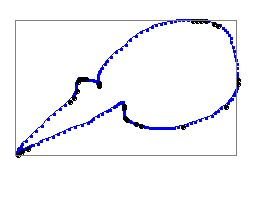
\includegraphics[scale=0.5]{images/stroke3.jpg}
	\caption{Input Stroke} Example of an input stroke to the system. 
	\label{fig:orignalStroke}
\end{figure}

 \begin{figure}
	\centering
			\subfigure[Speed versus Displacement Graph]{	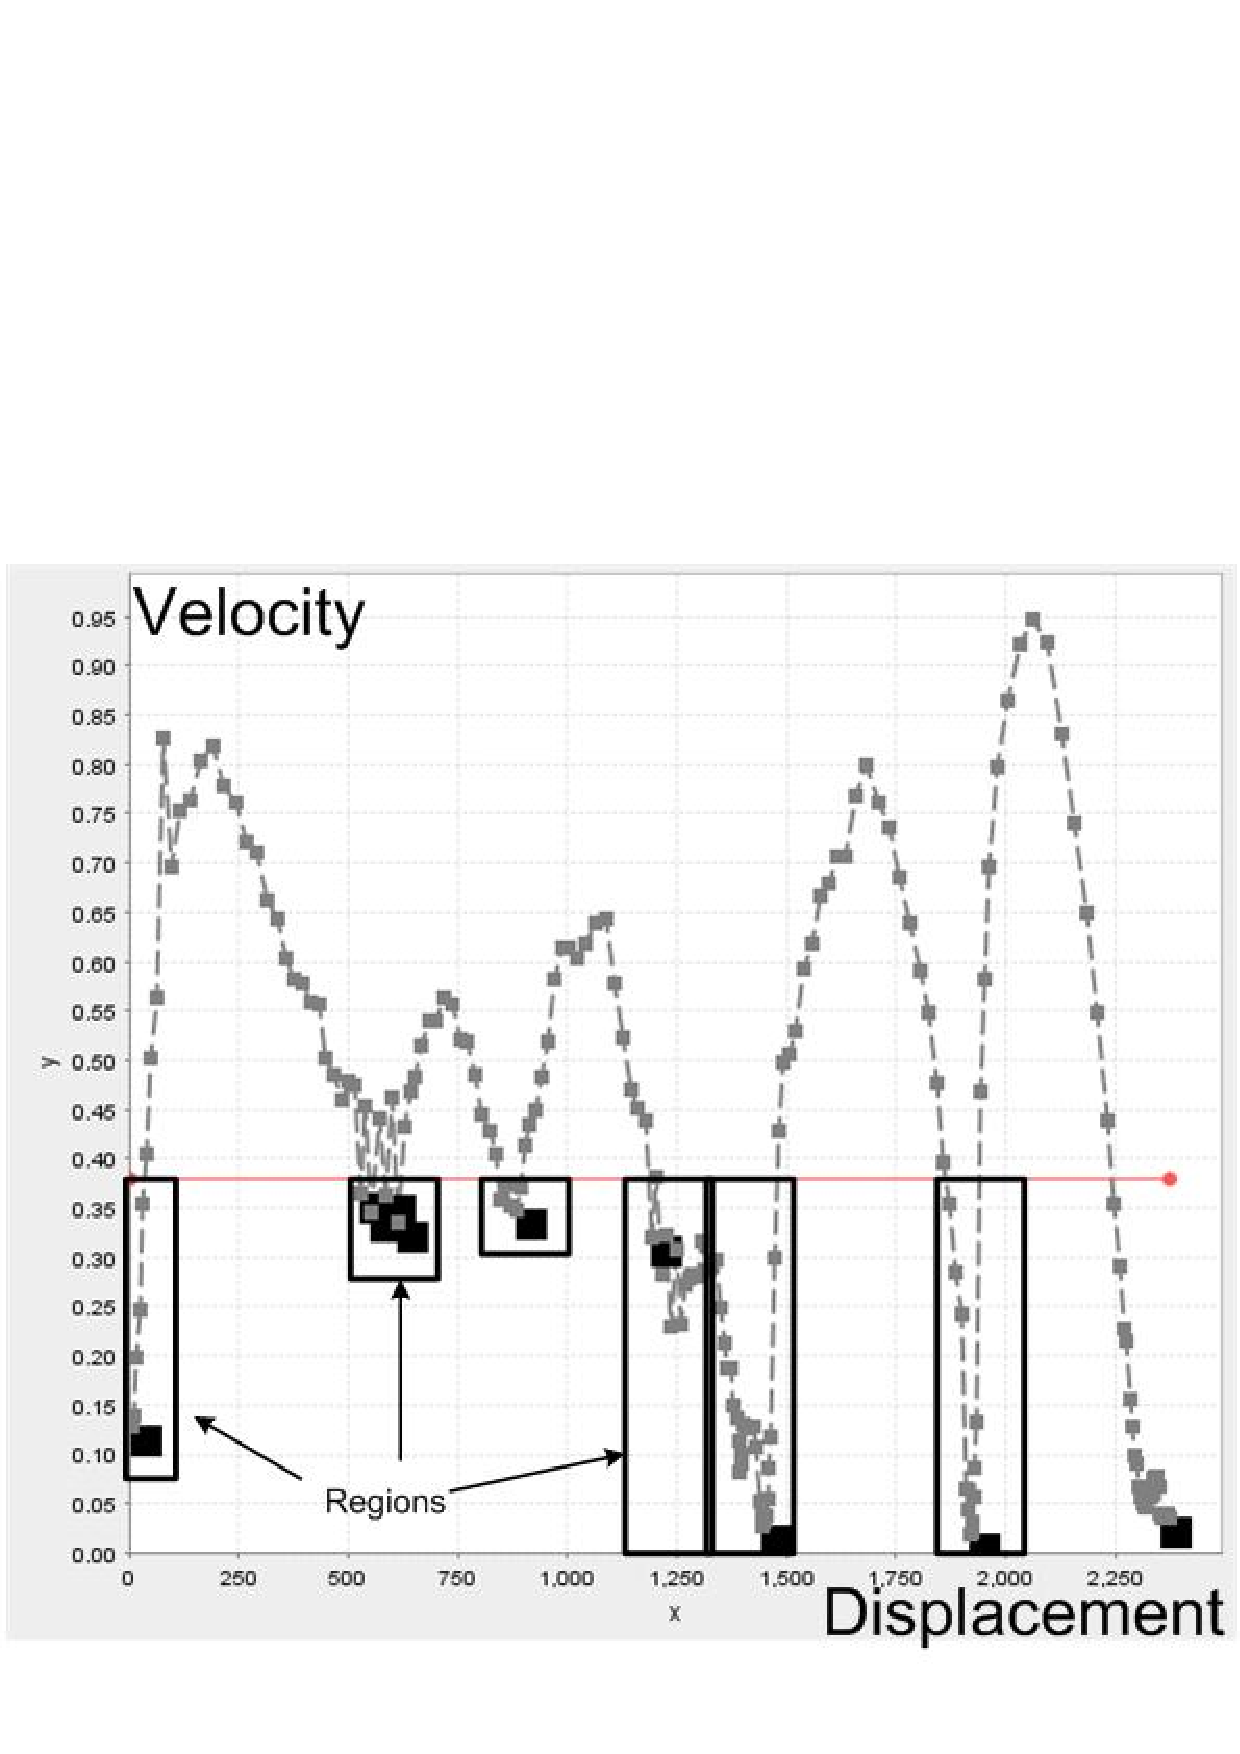
\includegraphics[scale=0.4]{images/vel3.jpg}}
			\hfill
			\subfigure[ Time Difference  versus Displacement Graph] {\label{fig:timediff}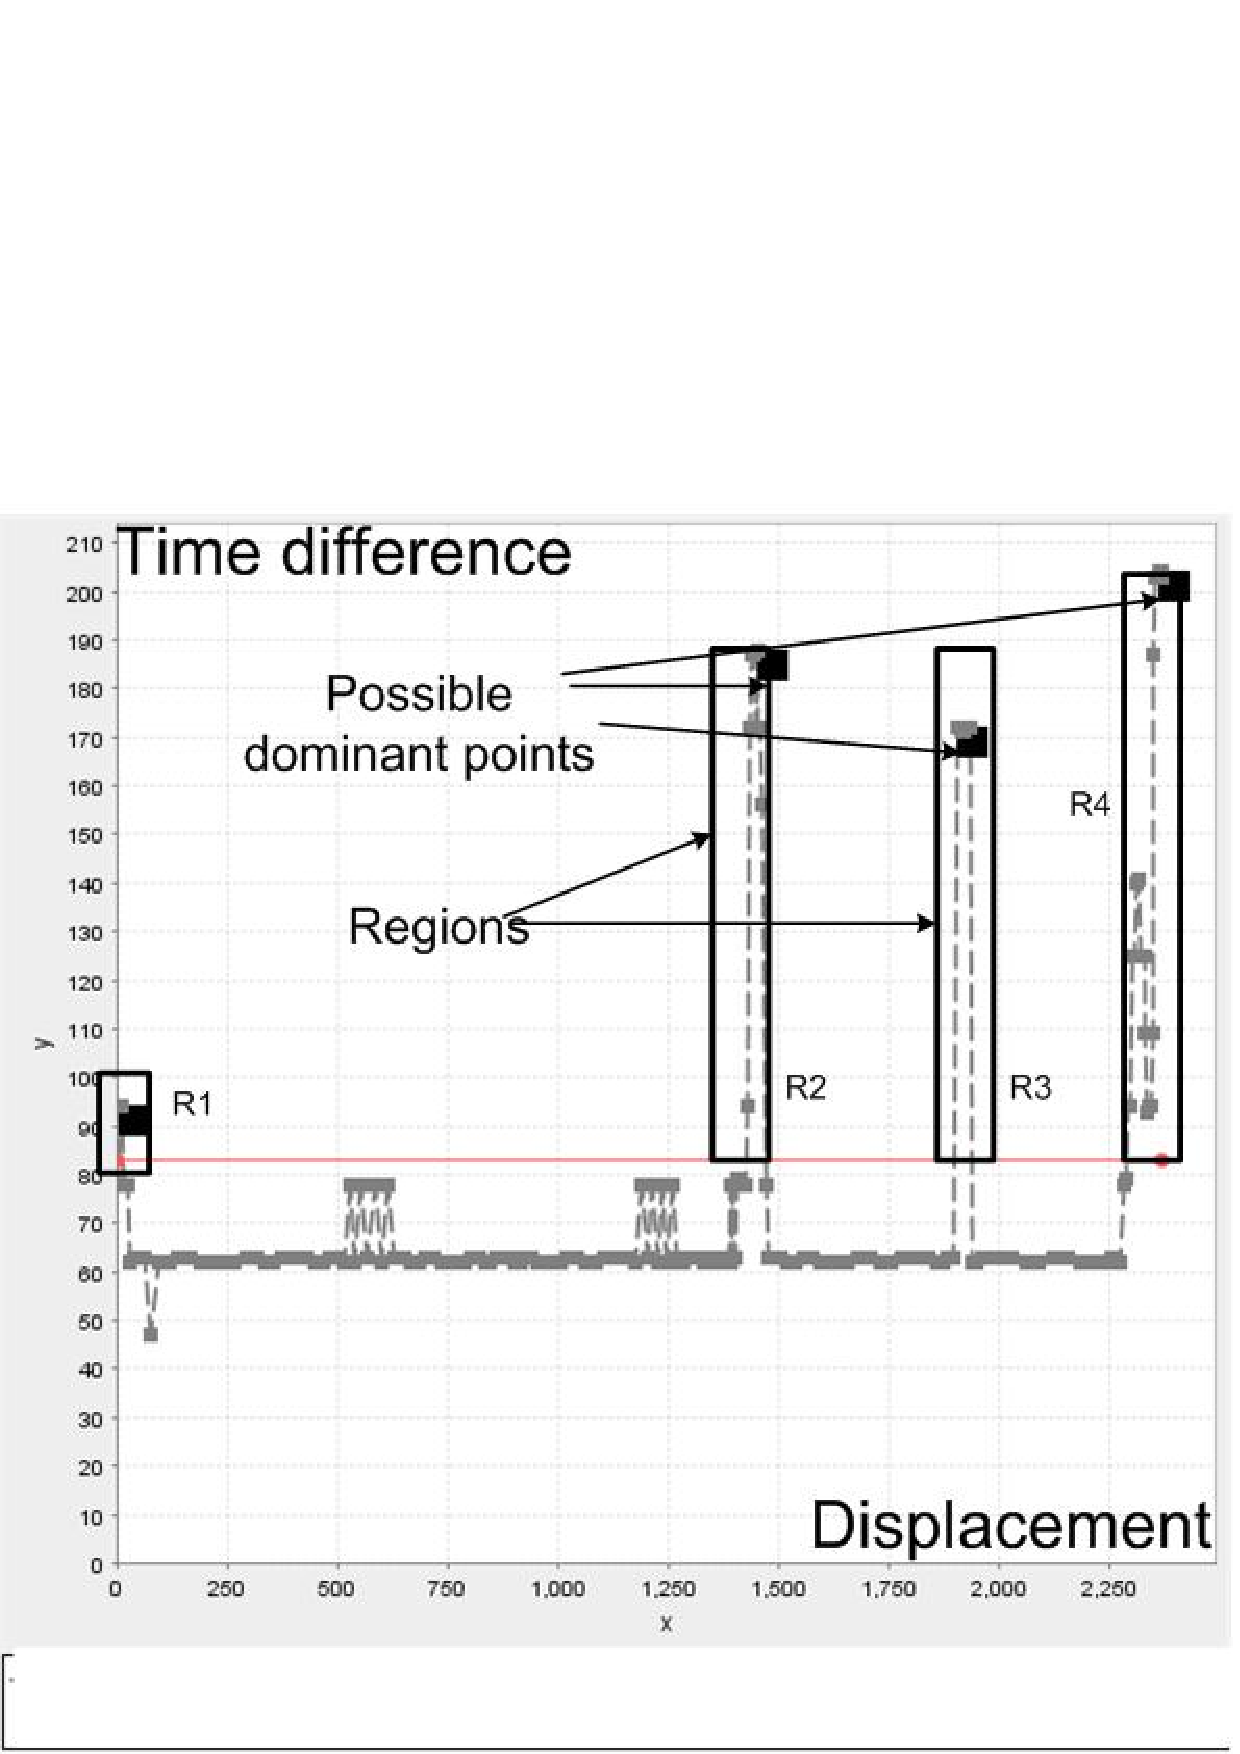
\includegraphics[scale=0.4]{images/td3.jpg}}
	\caption{Speed and Time Difference Graphs}  a) speed graph has lot of noise in the data with respect to b) time difference.   The black points denote the location of the possible dominant points $P_{pd}$. Black rectangles represent regions $R_i$ that in a) are lower than the thershold. b) are above the thershold. 
	\label{fig:speed2Distance}
\end{figure}
%is calculated as the angle between two vectors and  where $Q_i=\overrightarrow {P_{i - 1} P_i }$ is the vector from the point $P_{i - 1}$ to point $P_i$ 
Dominant points are characterized by low speed values, high curvature and direction values. However, the dominant points from the curvature information may not be the same points as the dominant points extracted from the speed information. Hence, we compute time difference, direction, speed and curvature of each point along a stroke to ensure that no dominant point is overlooked in this phase. The speed is calculated as $v=\Delta s/\Delta t$ where $t$ is the time difference between two points and $s$ is the length between them. The direction $d$ calculated as the angle between vectors $\overrightarrow {P_{i - 1} P_i }$ and the $x-axis$ and the curvature is considered as the change in direction $d$ with respect to length $s$ i.e. $c= \Delta d/\Delta s$. 
  
After the system computes the speed, time difference and curvature information, it proceeds to detect the points that have low velocity and high curvature. However, using simple differentiation to detect local extreme points results in false points due to the non smooth curves. Hence, our system adopted a process presented by \cite{earlyprocess}, where the mean of each of the four calculated information  is calculated. This mean is taken as the threshold \textit{th} which is used to separate the curve into regions ($R_i$) (Figure\ref{fig:timediff}); each region $R_i$ is defined as a range of points, where the curve values are either above or below the threshold \textit{th}. Those regions are further processed to find the maximum point $Max(R_i)$ of each region $R_i$. The stroke points $p_i(x,y)$ that correspond to those maximum values are labeled as \textit{possible dominant points} $P_{pd}$. The system repeats this process for curvature, time difference and speed information. All the points labeled as possible dominant points $P_{pd}$ are saved into a single array. Figure \ref{fig:ppd999} shows the particles labeled as Possible dominate point $P_{pd}$ in the preprocessing phase. It is clear that some of the $P_{pd}$ points are redundant as specified in the preprocessing stage. % (as shown are redundant)
\begin{figure}
	\centering
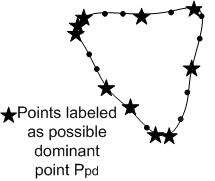
\includegraphics[scale=0.7]{images/ppd.jpg}
	\caption{Possible Dominante Points} An illustration of stroke points and the expected \textit{possible dominant points} $P_{pd}$.  
	%\label{fig:ppd}
	\label{fig:ppd999}	
\end{figure}

\subsection{Segmentation}
\label{seg}
In the segmentation stage, the input stroke is divided into a set of primitives. As shown in Figure \ref{fig:segblock} first an attempt is made to fit the stroke points into a curve or an ellipse using a minimum square error fitting algorithm \cite{ellipsefit}. The ellipse fitting step mainly helps to prevent the system from over segmenting the stroke into multiple lines or curves if the input stroke is an ellipse. If the stroke proved to be an ellipse arc then the segmentation process ends and the system proceeds to the next step. Otherwise, the stroke is passed to two further segmentation algorithms that divide the stroke to either lines or lines and curves. Hence we generate two different segmentations, the system chooses the segmentation with the minimum error. The following sections describe in details the ellipse detection algorithm and the two segmentation algorithms used to divide the stroke. % The input to these algorithms are the stroke points along with the possible dominant points $P_{pd}$ computed during preprocessing. The output is a set of dominant points which are connected by either lines or curves. 
%After two different segmentations are generated, 
%///AllBlockDiagram.jpg  you can change the block to the main block. 
 \begin{figure}
	\centering
		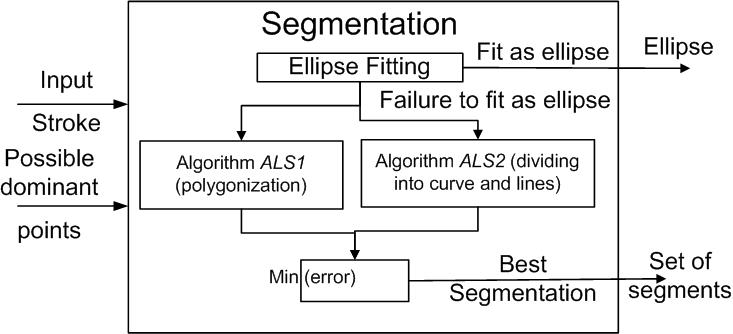
\includegraphics[scale=0.48]{images/blockSmall.jpg}
	\caption{Segmentation Block} 
	\label{fig:segblock}
\end{figure}
\subsection{Ellipse fitting}
%The process starts by computing the center of the stroke bounding box. The bounding box center point is used as the first estimation of the ellipse center. The axes of the ellipse are estimated as $width/2$ and $height/2$ of the stroke bounding box. The least square fitting algorithm is used to minimize the fitting error of the ellipse equation \cite{chernov}.  
This process attempts to fit the stroke points into an ellipse arc; it starts with computing the center of the stroke bounding box. The bounding box center point is used as the first estimation of the center of the ellipse. The axes of the ellipse are estimated as the $width/2$ and $height/2$ of the stroke bounding box where $width$ and $height$ are the width and height of the bonding box. The least square fitting algorithm \cite{chernov} is used to minimize the fitting error of the ellipse Equation (\ref{eq:circleFit})  
\begin{equation}
E = \sum\limits_{i = 0}^N {\frac{{(x_i - x_0 )}}{{a^2 }}^2  + \frac{{(y_i - y_0 )}}{{b^2 }}^2  - 1} 
\label{eq:circleFit}
\end{equation}
where $N$ is number of points in the stroke, $a$ \& $b$ are the length of ellipse axes, $x_0$ \& $y_0$ are the coordinates of the center point and $x_i$ \& $y_i$ are the coordinates of point $i$ in the stroke. A list of new values for $x_0$ , $y_0$ ,$a$ and $b$ are generated randomly from the older values with small increments after each loop.  After few iterations, the final fit error of the estimated ellipse is reported. Another measure is used to compute the efficiency of the final estimated ellipse. Equation \ref{eq:circleError} ensures that the drawn percentage of ellipse is considered. This eliminates fitting a  line into very large ellipse but leaves small ellipses to be fitted as a partial or a full ellipse. 

 \begin{equation}
%eff= (P_{percent}/E)
%eff = \left\{ {\begin{array}{*{20}c}
%   {\frac{{P_{percent} }}{E}} & {ifP_{percent}  < 0.5}  \\
%   {\frac{{P_{percent} }}{{E \times 2}}} & {ifP_{percent}  \ge 0.5}  \\
%\end{array}} \right,
eff= \begin{cases} 
\frac{P_{percent}}{E},&if P_{percent}< 0.5 \\
\frac{P_{percent}}{2\times E},&if P_{percent}\geq 0.5 \\
% \frac{P_{percent}}{2\times E},&\mbox{if} P_{percent}\mbox{\geq0.5} 
\end{cases},
\label{eq:circleError}
\end{equation}
 where $E$ is the error computed by Equation (\ref{eq:circleFit}), and 
\[
P_{percent}  = L_{stroke} /P_{ellipse}, 
%\label{eq:ErrorArea}
\]
 where $L_{stroke}$ total length of stroke and $P_{ellipse} $ is the perimeter of the estimated ellipse. If $eff$ has a value more than threshold $th_{Ellipse}$\footnote{By trial and error best threshold found was $th_{Ellipse}=0.2$} then the stroke is segmented as an ellipse otherwise the system proceeds to the next step. 

\subsection{Non ellipse fitting algorithm}
\label{subsubsec:Discreteparticleswarmalgorithm}
\begin{figure}
	\centering
		%\subfigure[Possible dominate point]{ 	\label{fig:LabelsPPD}	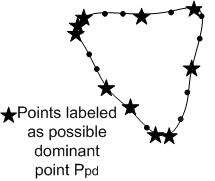
\includegraphics[scale=0.7]{images/ppd.jpg}}
	%	\hfill
	 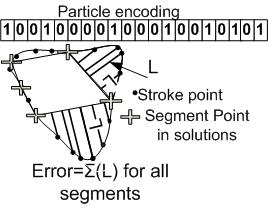
\includegraphics[scale=0.7]{images/pso1.jpg}			
	\caption{DPSO algorithm encoding} The swarm particle encoding where 1 represent the dominant points or segment points (i.e points are drawn as a big plus). Length L is the distance between a stroke point and the line connecting two successive segment points. %represent the length   % a) Possible dominate point b) Particle encoding  
	\label{fig:pso1}
\end{figure}
Two DPSO algorithms are used to generate different segmentations for each stroke the user draws. For each segmentation generated, an error is evaluated. The segmentation with the minimum error value is chosen as the best stroke segmentation (Figure \ref{fig:segblock}). The problem definition is the same in both algorithms but they differ in the method they use to compute fitness and error functions. 
\begin{description}
	\item[ Problem definition:] The input stroke $S$  with $N$ points can be represented by set $S = \left\{ {x_1 ,x_2  \ldots x_N }\right\}$ where $x_i$ is the location of the point $i$. The swarm algorithms consist of $M$ agents which are represented by the set $A = \left\{ {P_i \left| {i = 1,2 \cdots M} \right.} \right\}$ where $P_i$ is a single solution particle from the solution space. Each particle decodes the problem using a binary array with the same length $N$ as the input stroke.  

Therefore, the system represents each particle $P_i$ by $P_i = \left\{ {p_{ij} \left| {j = 1,2 \cdots N} \right.} \right\}$ where $p_{ij}$ has only two values a)1 ($p_{ij}=1$); means that this point ($j$) is a dominate point, or b) 0 ($p_{ij}=0$) means this point ($j$) is not a dominate point. Figure\ref{fig:pso1} shows a particle encoding in the DPSO system. 

	\item[Fitness function:] The fitness function and error calculation are different in each of the two \textit{DPSO} algorithms. 
	\end{description}
\subsubsection{\textit{Polygon Approximation Algorithm \textsl{(AlgS1)}}}
%\\
The approximation error is computed by the equation \ref{eq:ErrorSwarm1}. The graphical meaning of the error is shown in Figure\ref{fig:LabelsPSO}.
\begin{equation}
E=\sum\nolimits_{i = 0}^M e ( \widehat{x_ix_{i+1}},\overline{x_i x_{i+1}})
\label{eq:ErrorSwarm1}
\end{equation} where the arc $\widehat{x_ix_j}$ is defined as the consecutive set of points from point $x_i$ to point $x_{j}$ as in $x_i,x_{i+1} \cdots,x_j$. The line $\overline{x_i x_j}$ is defined as the straight line connecting point $x_i$ to point $x_j$ and $M$ is the number of dominant points in this solution as generated by the swarm algorithm. The error $e ( \widehat{x_ix_j},\overline{x_i x_j})$ is computed as the sum of squared perpendicular distance from every point along the arc $\widehat{x_ix_j}$ to the line $\overline{x_i x_j}$. The fitness is computed using the following equation %\ref{eq:fitnessSwarm1}
\begin{equation}
\max fitness(p_i ) = \left\{ {\begin{array}{*{20}c}
   {\frac{-E}{\varepsilon N}} & {ifE > \varepsilon ,}  \\
   
   {D/\sum\limits_{j = 1}^N {p_{ij} } } & {otherwise}  \\
\end{array}} \right.
\label{eq:fitnessSwarm1}
\end{equation} where $N$ is the number of points in the stroke, $D$ is the number of points in the solution that was previously labeled as a possible dominant point ($P_{pd}$), $E$ is the computed error and $\varepsilon$ is the error threshold. It should be noticed that when the error is larger than the threshold $\varepsilon$ the fitness is given a -ve value to lower the fitness value of the solution. Otherwise the system favors the lower number of vertices.

 \subsubsection{\textit{Hybrid Fitting \textsl{AlgS2}}}
The algorithm has the same problem formulation but different fitness and error functions are used. An attempt is made to fit each segment into a line or circular arc. The errors of both circle and line fit estimations are computed for each segment $S_i=\widehat{x_ix_j}$. The approximation with the lower error value is chosen as the final approximation of this segment $S_i$\cite{CruveDivisionSwarm}. The sum of the approximation errors of all segments is the total error of the particle.  The total error of the particle is computed by equation %\ref{eq:errorSwarm2}
 \begin{equation}
E=\sum\nolimits_{i = 0}^M e(D_i) 
\label{eq:errorSwarm2}
\end{equation}where $M$ is the number of segments in the solution as generated by the swarm algorithm, $D_i$ is the minimum approximation error of curve and line approximations $min(d_c,d_l)$ where $d_c$ is the circle approximation error and $d_l$ is the line approximation error as computed by \cite{CruveDivisionSwarm}.  The fitness is computed by the equation %\ref{eq:fitnessSwarm2} 
\begin{equation}
\max fitness(P_i ) = \frac{1}{{E \times M^k }}
\label{eq:fitnessSwarm2}
\end{equation} where $E$ is the error and $M$ is the number of segments and $k$ is a parameter tweaked to get minimum number of segments. The larger $k$ is, the more effect the number of segments will have. For our system, $k$ is selected to be 0.5\cite{CruveDivisionSwarm}.

After each iteration of the swarm algorithm (\textsl{AlgS1} and \textsl{AlgS2}), each particle is refined using the following procedures: 
\begin{enumerate}
	\item For each particle $P_i$ each dominant point $P_{ij}$ is checked to find if it was labeled before as a \textit{possible dominant point} $P_{pd}$ (computed as in section \ref{Prepross}). If it was not labeled the point $P_{ij}$ is moved to the nearest labeled point. This ensures that all of the points generated by the DPSO are possible dominant points $P_{pd}$. 
	\item The particles are tested to make sure that the distance between every two successive dominate point is larger than $min_D$, where $min_D$ is 5\% of the total length of the stroke.  Otherwise, one of these points are removed based on the error cased by its removal.
	\item Each two successive segments are test to determine if they can be merged into a single segment. If merging the two segments have the same or smaller the error, the two segments are merged. This step ensures that the final segmentation of the system has minimum number of segments. 
\end{enumerate}
%1) 2)  % If two points are nearer than $min_D$ then one of the points is removed. 
\subsection{Recognition}
\label{sec:Recognition}
After the user draws all strokes of the symbol, the set of un-recognized strokes is grouped together along with their segmentation as input to the feature extraction process. A composite set of features is used to generate a single feature vector. The following list describes each feature in details.
%\begin{description}
\subsubsection{Structural and geometrical Features(FS1)}
  Features defines the structure of the geometrical symbol.  
%\begin{description}
%	 \item[No. Of segments] Number of segments in the symbol. 
%		\item[No. Of primitives] Number of primitives in the symbol. The feature helps when identifying             symbols with mixed geometric primitives like cylinders and callouts.  
%		\item [No. of curves] Number of curves or ellipses in the symbol. 
%		\item [No. of lines] Number of lines in the symbol. 
%		\item [No. of perpendicular lines] Number of perpendicular lines. 
%		\item [No. of parallel lines] Number of parallel lines. 
%		\item [No. of intersections] Number of intersection between lines and curves. 
%		\item [Size Ratio] Ratio between width to height of the symbol.
%		%\item[No. of holes] Number of holes in the symbols. 
%
%\end{description}
 \begin{itemize}
	 \item \emph{Segments:} Number of segments in the symbol.
	 \item \emph{Strokes:} Number of strokes or partial strokes that created the symbols.  
		\item  \emph{Primitives:} Number of primitives in the symbol. The feature helps when identifying             symbols with mixed geometric primitives like cylinders and callouts.  
		\item \emph{Curves:} Number of curves or ellipses in the symbol. 
		\item \emph{Lines:} Number of lines in the symbol. 
		\item \emph{Perpendicular} lines Number of perpendicular lines. 
		\item \emph{Parallel} lines Number of parallel lines. 
		\item \emph{Intersections} Number of intersection between lines and curves. 
		\item \emph{T intersections} Number of T intersections. 
		\item \emph{L intersections} Number of L intersections. 
		\item \emph{X intersections} Number of X intersections.
	
		%\item[No. of holes] Number of holes in the symbols. 
\end{itemize}
\subsubsection{Rubine Feature Set (FS2)}
  Features introduced by Rubine\cite{gestureexample12} for single stroke gestures. Feature such as length of stroke, smoothness of symbol and properties of the bounding box of the symbol. 
  
\subsubsection{Statistical Features (FS3)}  
\begin{itemize}
	\item \emph{Zernike moments } Zernike moments of order n (10 or 20).  \cite{HeloiseBeautification}. 
\end{itemize}
\subsubsection{Composite Features (FS4)}
 Features that are composites of different geometrical and statistical symbol. 
	\begin{itemize}
\item \emph{Size Ratio} Ratio between width to height of the symbol.
	\item \emph{Ink density} Compute the density of points inside its bounding box\cite{GeometryAndDomain102}.   
 	\item \emph{Convex Hull Area} Area of convex hull with respect to area of bounding box of symbol.
	\item \emph{Convex Hull Perimeter} Perimeter of convex hull with respect to total length of symbol.
		\item \emph{Mean Centroidal radius} The Mean of the centroidal radius which is the distance from each point in the symbol to the center of gravity.
	
	\item \emph{Mean Time difference} The mean of the time difference between each two successive points in the symbol. %Different strokes are appended to construct a single path.
	%\item [Ra]
  \end{itemize}
  
  
%\end{description}
%The features used consist of Rubine feature set,  of order 21 , ink density as well as some structural and spatial information like number of perpendiculars lines ,number of parallel lines and number of different types of primitives in each symbol. 
After computing the features the symbol is introduced to the classifier. The system uses Support Vector Machine (SVM) classifier with Linear kernel \cite{libsvm}. An OVO classifier structure (object versus object) is used to handle multi-class.% A validation algorithm is used to choose the Kernel variables parameters $c, \gamma$.

\section{Experimental}
\label{sec:Experiments}
In our experiment we used three different datasets. First dataset was collected by Hse and Newton\cite{HeloiseBeautification} (Hs-DB). The data are drawn by 16 users each of them was asked to draw 13 shapes from 30 to 50 times. Figure \ref{fig:symbolSet} shows a set of the shapes used in the data set. We collected the second and third datasets. Figure \ref{fig:ELsymbolSet} and \ref{fig:LogicsymbolSet} shows the symbols gathered from 7 different users in electrical (EL-DB) and logic design (LD-DB) domain respectively.  Table \ref{tab:datasets} shows a  comparison between the three datasets used in our experiments. The datasets were divided into training set and test set. Five different splits  for the training and test data are generated from each dataset. The results displayed are the average recognition accuracy of the five splits. The accuracy is computed as the number of correctly recognized samples divided by the total number of samples in the test. 


\begin{figure}
\centering 
\label{fig:symbolSet}
\fbox{ \parbox{5cm}{% 
		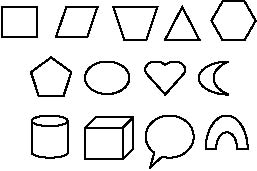
\includegraphics[scale=0.5]{images/symbolSet.PNG}	}}
		\caption{The Hs-DB Symbol Set}.
\end{figure}
\begin{figure}
\centering 
\label{fig:LogicsymbolSet}
 
		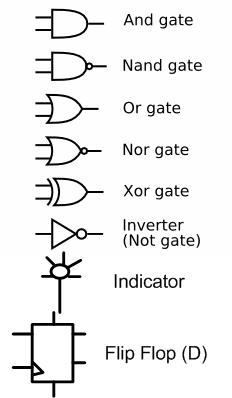
\includegraphics[scale=0.5]{images/logicSet.jpg}	 
		\caption{The Digital Design Symbols Dataset(LD-DB)} Symbols used in the dataset.
\end{figure}
\begin{figure}
\centering 
\label{fig:ELsymbolSet}
\fbox{ \parbox{4.5cm}{% 
		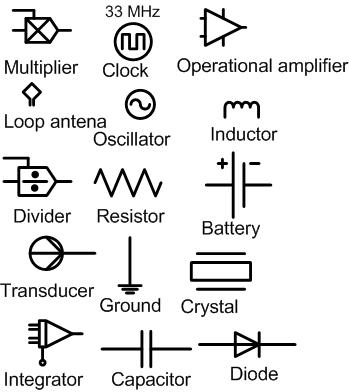
\includegraphics[scale=0.5]{images/EelectImage.jpg}	}}
		\caption{The Electrical Symbols Dataset(EL-DB)} .
\end{figure}


\begin{table}
\begin{center}
\scalebox{0.9}{
 \begin{tabular}{|p{2cm}|p{1.5cm}|p{1.5cm}|p{1.5cm}|}
 \hline
 & Hs-DB &  EL-DB & LD-DB \\ \hline
No of samples  &  7791 & 2764 & 1859 \\ \hline
No of categories  & 13 & 15 & 8 \\ \hline
Avg. Samples per Category& 600 & 184 & 232 \\\hline 
No of users  & 16 & 7 & 7 \\  \hline
Balanced & Yes&No & No \\ \hline
Splits  & 5 random splits  & 5 random splits  & 5 random splits  \\ \hline
Examples & Figure \ref{fig:symbolSet}  & Figure \ref{fig:ELsymbolSet}  & Figure \ref{fig:LogicsymbolSet}   \\ \hline
\end{tabular}
}
\caption[Datasets Comparisons]{Datasets Comparisons} 
\label{tab:datasets}

\end{center}
\end{table}

 

%The dataset collected by Hse and Newton\cite{HeloiseBeautification} is used to test the presented system. The data are drawn by 16 users each of them was asked to draw 13 shapes from 30 to 50 times. Figure \ref{fig:symbolSet} shows a set of the shapes used in the data set. The dataset was divided into training set and test set. Four different splits for the training and test data are generated from the dataset. The results displayed are the average recognition accuracy of the four splits. The accuracy is computed as the number of correctly recognized samples divided by the total number of samples in the test. %In the following section, the recognition accuracy means the average recognition accuracy in the four data splits.  

\subsection{Algorithms comparisons}
\label{sec:AlgExp}
A set of tests were performed on the system to enhance non ellipse fitting algorithm. The effect of number of agents, the error thresholds and various other parameters were investigated. The result of these tests are shown in Figure \ref{fig:swarmtesting} and   \ref{fig:swarmtesting2}. Figure \ref{fig:swarmtesting} shows that as the number of agents increases the error value decrease (error of the segmentation algorithm). The final number of agents and maximum swarm iteration used in the system was based on a trade off between error achieved versus the computation time. Other algorithm parameters such as $c_1$,$c_2$ that were mentioned in Section\ref{sec:ParticleSwarmAlgorithm} are tested using similar tests (Figure \ref{fig:swarmtesting} and \ref{fig:swarmtesting2}).
    
 \begin{figure}
	\centering		
	 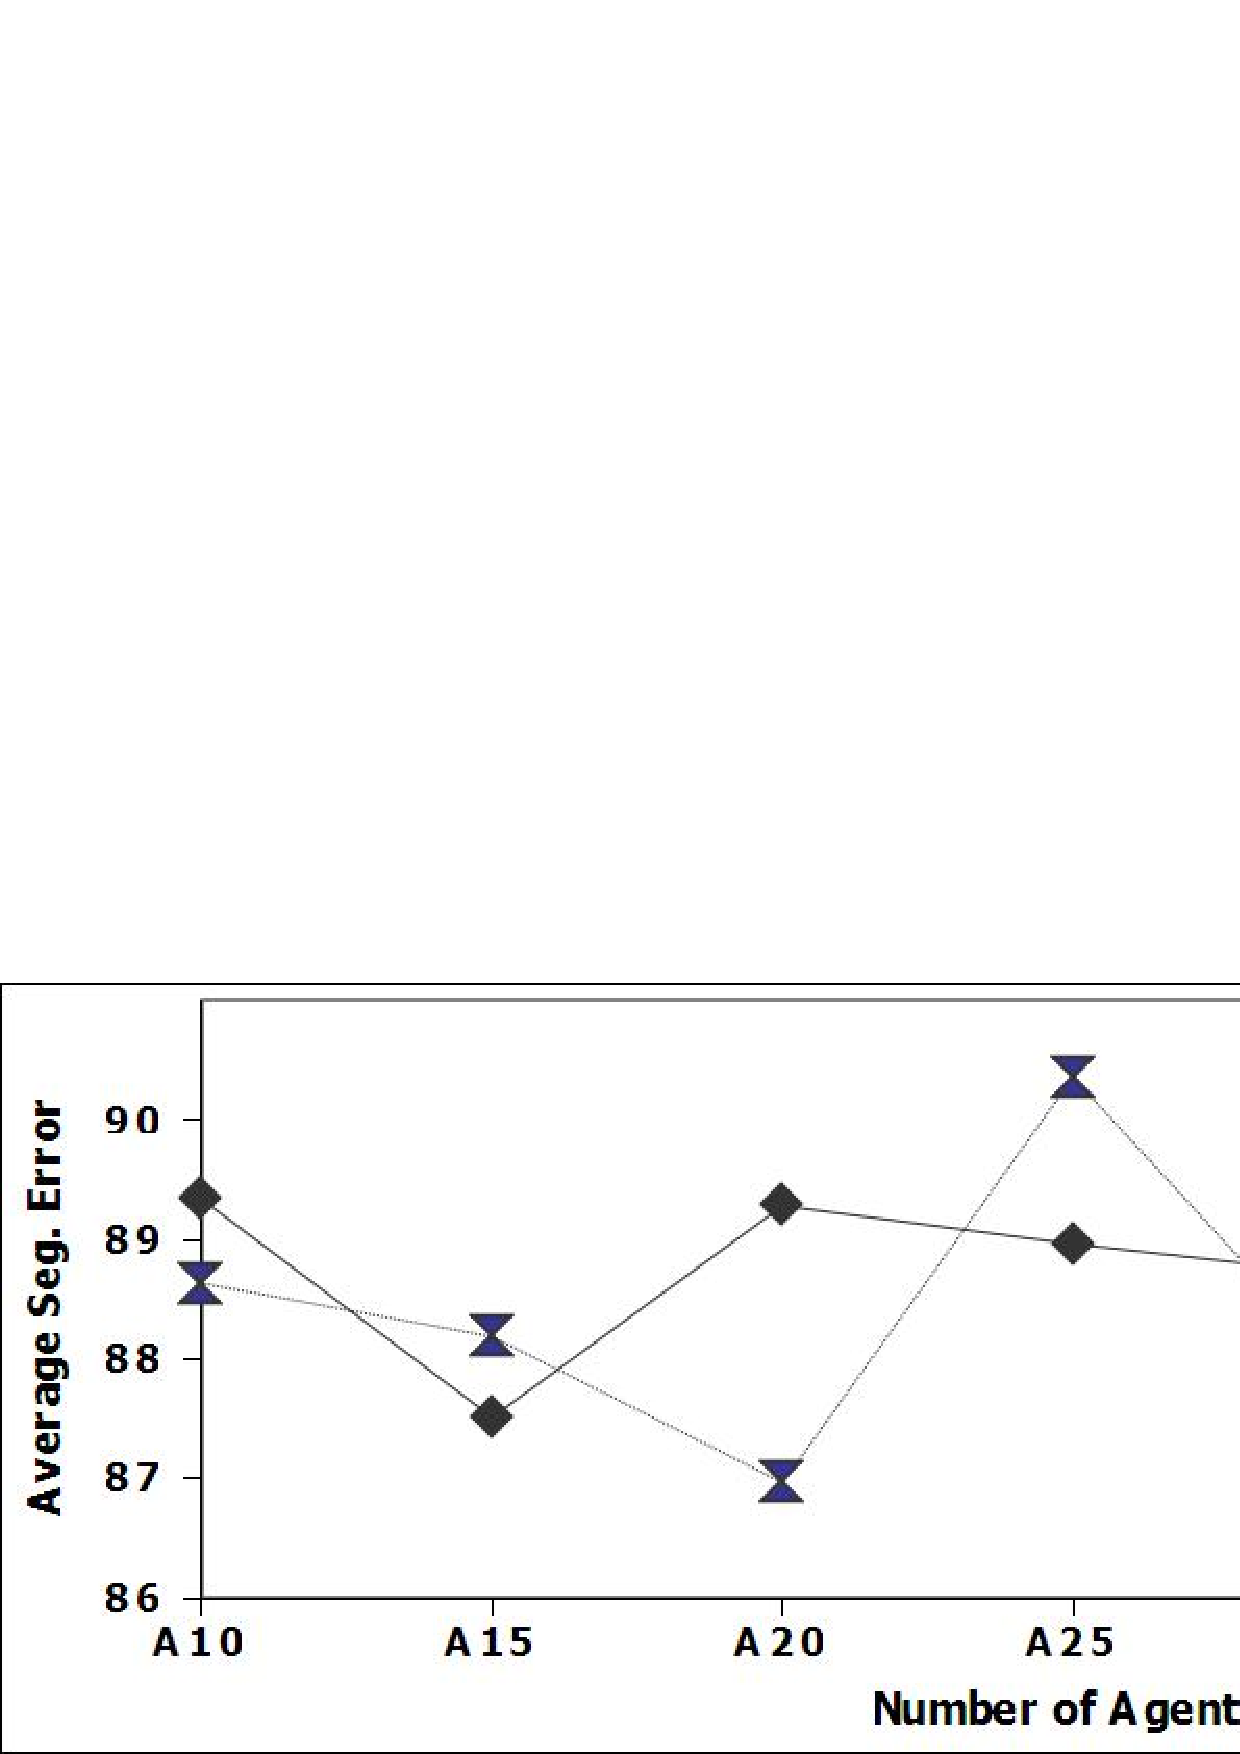
\includegraphics[scale=0.3]{images/swarmAgentTest.jpg}
	 	\caption{Swarm testing} Segmentation Error Vs. Number of agents
	 	\label{fig:swarmtesting}
	%\caption{Experiments results :} a)    b) c) 
\end{figure} 

\begin{figure}
	\centering		
	 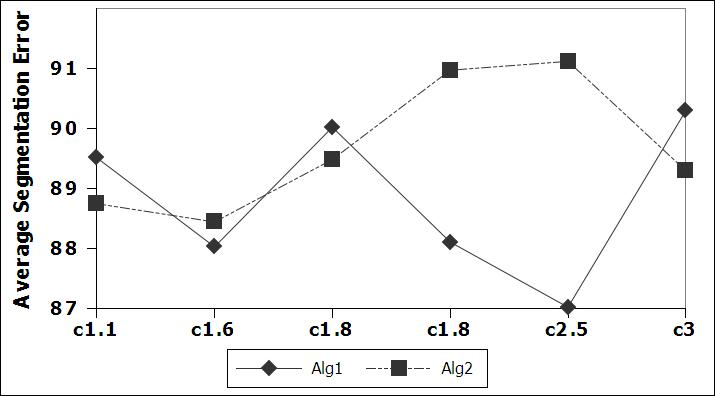
\includegraphics[scale=0.4]{images/swarmParamterC.jpg}
	 	\caption{Swarm testing} Segmentation Error Vs. PSO parameters.
	 	\label{fig:swarmtesting2}
	%\caption{Experiments results :} a)    b) c) 
	
\end{figure} 

We performed several experiments to evaluate the presented recognition system. Firstly we tested recognition accuracy of shapes in the data set with both algorithms (\textsl{AlgS1} and \textsl{AlgS2}). We also implemented the segmentation algorithm described in \cite{earlyprocess} (\textsl{Alg3}) to use as reference to compare it with our swarm algorithms. Figure \ref{fig:test1} and \ref{fig:testLD} shows the accuracy achieved by each algorithm. The two swarm algorithms were tested with and without the ellipse fitting module. The ellipse detection module appears to be superior. The result shows that combining both  (\textsl{AlgS1} and \textsl{AlgS2}) out perform any single algorithm. %show that combining algoirthmsachieve higher accuracy than any single algoirthm. 
%improves the results.% with both the \textit{DPSO} algorithms.% The results show that both \textit{DPSO} algorithms achieve better result than other algorithms. 

 \begin{figure}
	\centering		
	 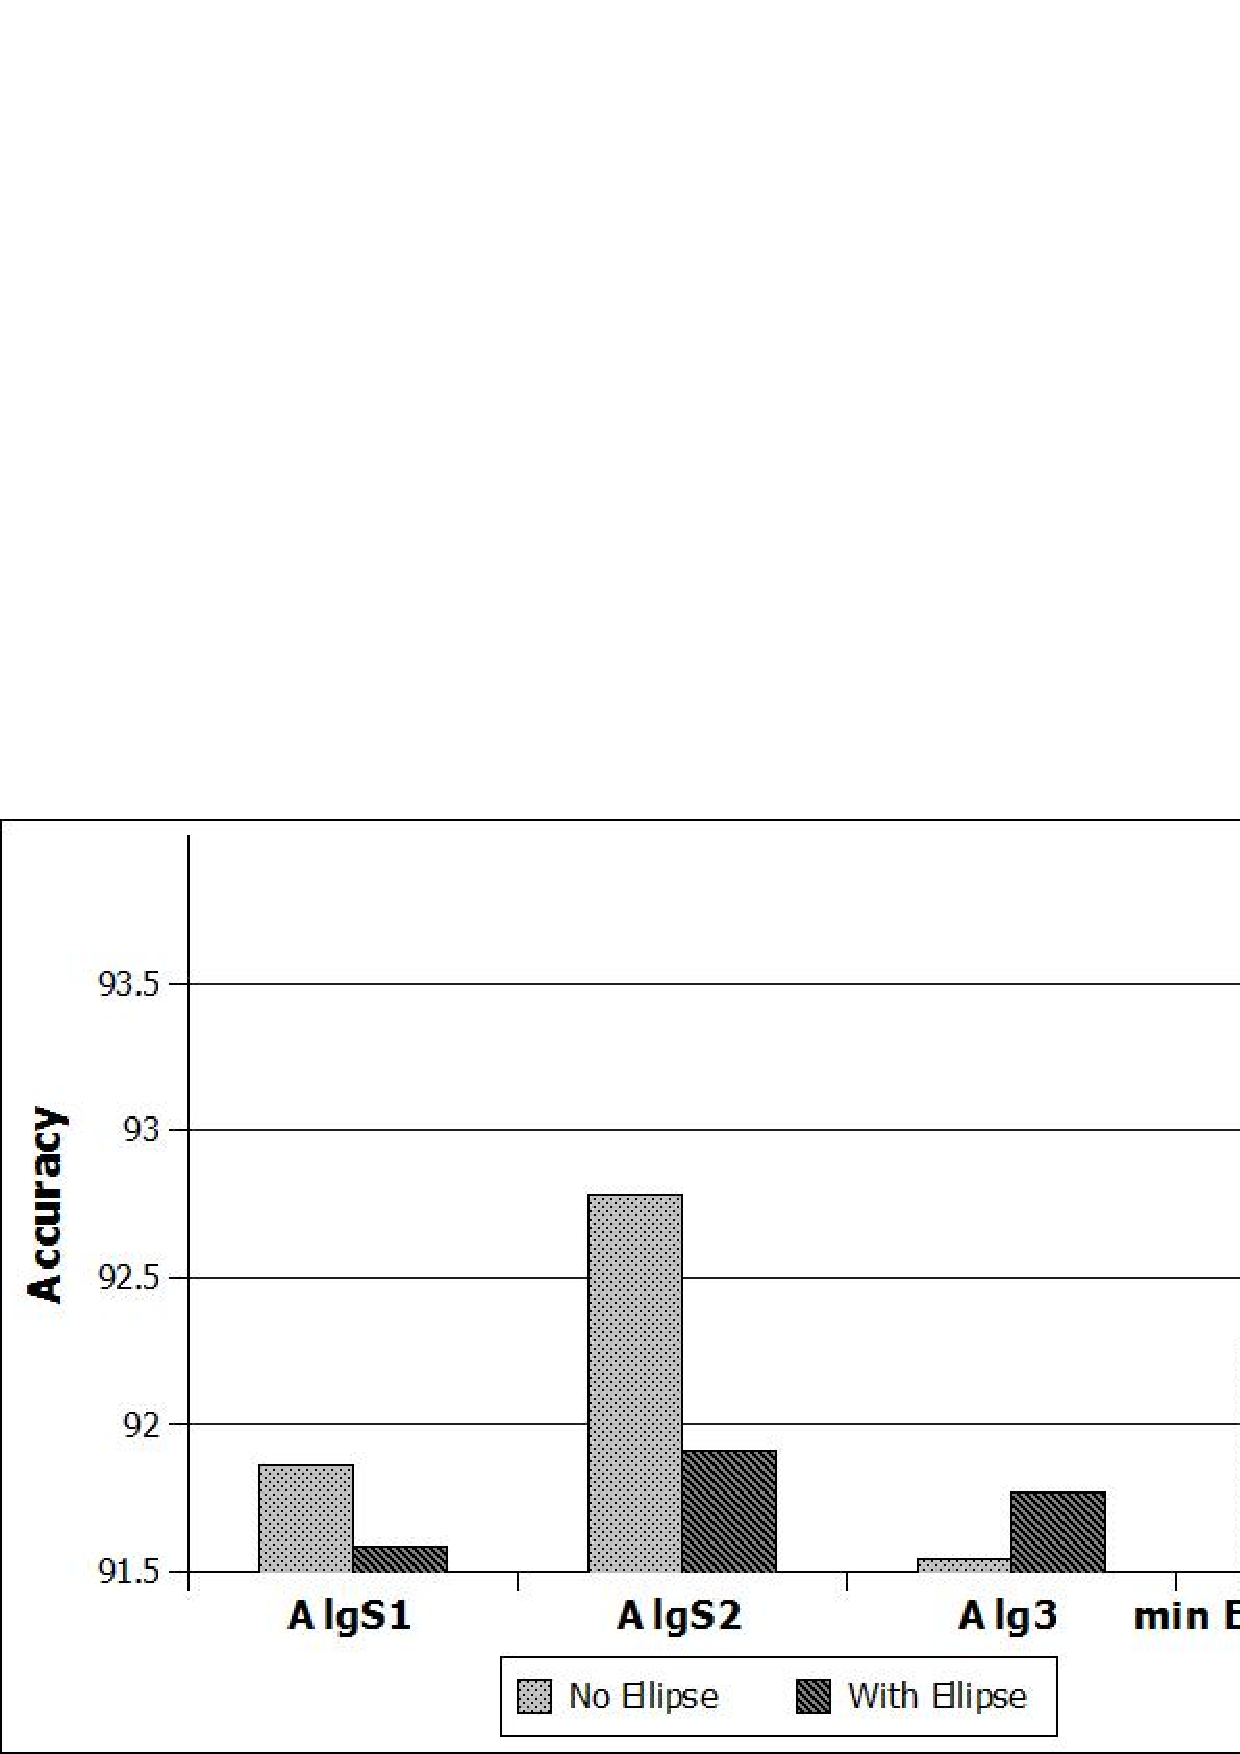
\includegraphics[scale=0.4]{images/testAlg.jpg}
	 	\caption{Algorithm comparison on HS-DB} The recognition rate of different algorithms. 
	 	\label{fig:test1}
	%\caption{Experiments results :} a)    b) c) 
\end{figure} 




\begin{figure}
	\centering		
	 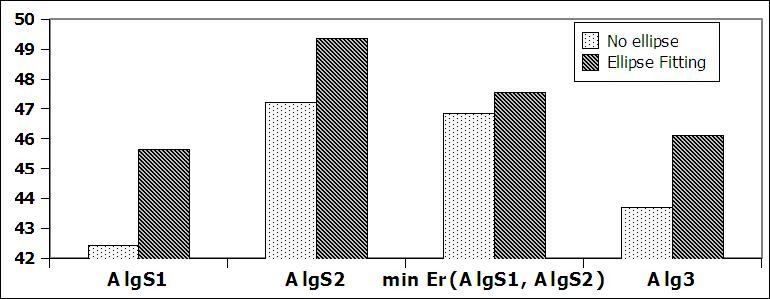
\includegraphics[scale=0.4]{images/LDAlg.jpg}
	 	\caption{Algorithm comparison on LD-DB} The recognition rate of different algorithms. 
	 	\label{fig:testLD}
	%\caption{Experiments results :} a)    b) c) 
\end{figure} 

\begin{figure}
	\centering		
	 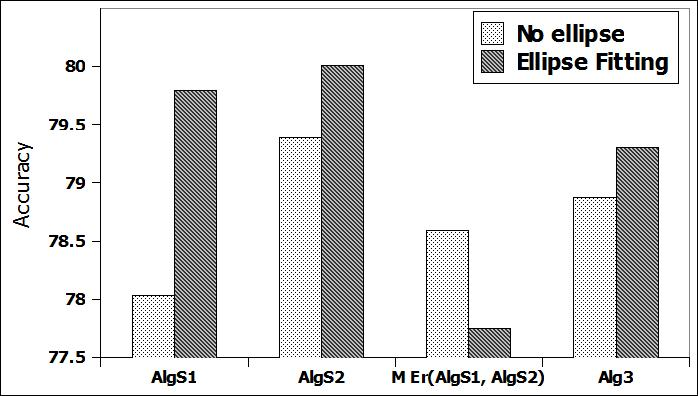
\includegraphics[scale=0.4]{images/AlgEL.jpg}
	 	\caption{Algorithm comparison on EL-DB} The recognition rate of different algorithms. 
	 	\label{fig:testEL}
	%\caption{Experiments results :} a)    b) c) 
\end{figure} 


\subsection{Shape Complexity Analysis}
\label{sec:ShapeComplexityExperiments}

\begin{figure*}
	\centering
		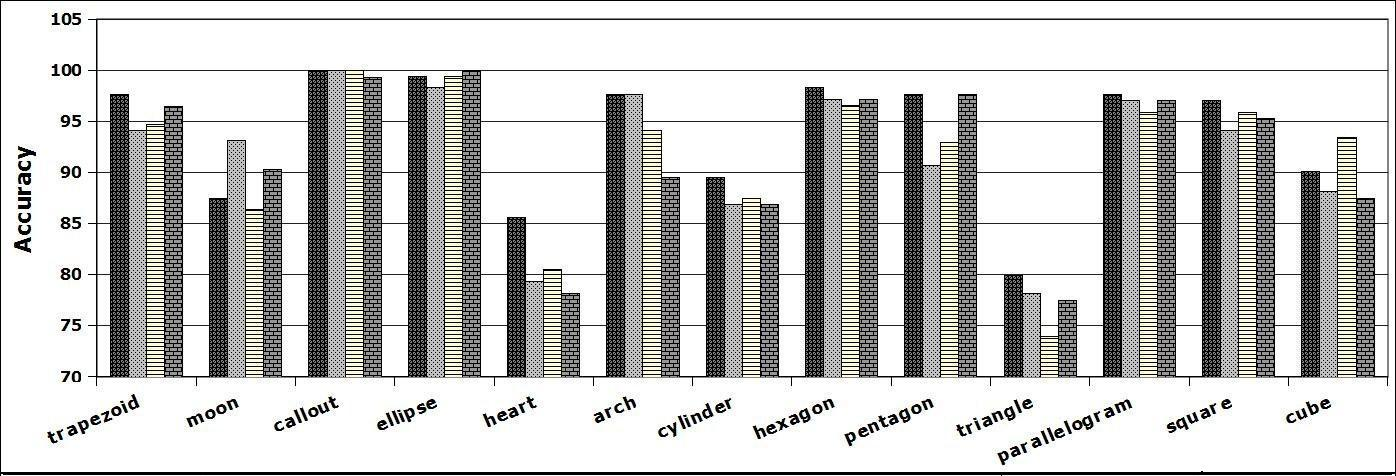
\includegraphics[scale=0.5]{images/testsym.jpg}
	\caption{Symbols Comparison on HS-DB} The effect of symbol complexity.  %The graph shows the recognition rate of each symbol using different algorithms. 
	\label{fig:test2}
\end{figure*}  

\begin{figure*}
	\centering
		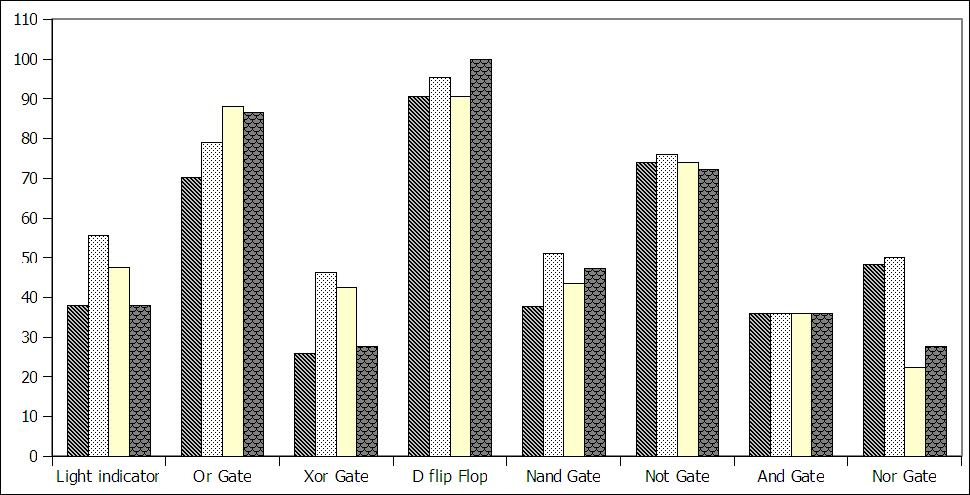
\includegraphics[scale=0.5]{images/LDsymbols.jpg}
	\caption{Symbols Comparison on LD-DB symbols}.  %The graph shows the recognition rate of each symbol using different algorithms. 
	\label{fig:LDtest2}
\end{figure*}  
The second experiment we implemented was to investigate the effect of symbol complexity and type on the recognition rate. Figure \ref{fig:test2} and \ref{fig:LDtest2} shows the achieved accuracy of each symbol by our algorithms compared to \cite{earlyprocess} (\textsl{Alg3}). It is clearly noted that symbols that have only line segments achieve higher accuracy rate than other symbols. The results indicate that algorithm \textsl{AlgS1} achieve better performance than algorithm \textsl{AlgS2} in the symbols that consist only of lines. This is understandable because algorithm \textsl{AlgS1} divides strokes into line segments only but \textsl{AlgS2} is able to divide strokes into lines and curves based on the minimum error of the segment itself. Figure \ref{fig:LDtest2} shows that in logic design symbols \textsl{AlgS2} achieved better performance than \textsl{Alg3} \textsl{AlgS1} this emphases that complex shapes that are combination of lines and arc are better segmented using \textsl{AlgS2}. Algorithm \textsl{Alg3} gives good performance as long as the symbols consist of combination of lines and curves, if the stroke consists of only curve or lines the algorithm may lead to wrong segmentation result. This is because the system divides the stroke first to line segments then tries to decide if each segment can be represent better as a curve unlike algorithm \textsl{AlgS2} where the curve segments are tested while choosing the best segmentation. Combining both algorithm \textsl{AlgS1} and \textsl{AlgS2} improved the recognition rate of all symbols. The penalty for this improved performance is the computational time required to run both swarm algorithms. Table \ref{tab:ConfusionMatrix} shows the confusion matrix of symbols. The table shows that errors are only between two sets of symbols moon with triangles and trapezoid with triangles. This observation is understandable as the symbols are visually similar but the system must be able to differentiate between them. This lead us to the next experiment to choose best set of feature to recognize symbols. 
\begin{table*}
	\centering
	%\small
%	\scalebox{0.7}{
		%	\begin{tabular}{|c|c|c|c|c|c|c|c|c|c|c|c|c|c|}\hline 
 %%%%%%%%%%%%%%%%%%%%%%%%%%%%%%%%%%%%%%%%%%%%%%%%%%%%%%%%%%%%%%%%%%%%%%
%%                                                                  %%
%%  This is a LaTeX2e table fragment exported from Gnumeric.        %%
%%                                                                  %%
%%%%%%%%%%%%%%%%%%%%%%%%%%%%%%%%%%%%%%%%%%%%%%%%%%%%%%%%%%%%%%%%%%%%%%
	\scalebox{0.5}{  % this was taken from algfeat from  Results_17-04-2009_07-13
			\begin{tabular}{|c|c|c|c|c|c|c|c|c|c|c|c|c|c|}\hline 
 Categories 	&ellipse	&heart	&trapezoid	&pentagon	&arch	&hexagon	&square	&triangle	&cube	&cylinder	&parallelogram	&moon	&callout\\ \hline 
ellipse	&150	&20	&0	&0	&0	&5	&1	&0	&0	&0	&0	&1	&0\\  \hline 
heart	&2	&130	&0	&1	&10	&1	&1	&0	&0	&0	&1	&4	&0\\  \hline 
trapezoid	&0	&1	&147	&5	&1	&0	&1	&3	&2	&0	&37	&0	&0\\  \hline 
pentagon	&0	&0	&1	&139	&0	&7	&0	&0	&0	&0	&1	&0	&0\\   \hline 
arch	&0	&0	&1	&1	&125	&0	&4	&0	&3	&0	&0	&15	&1\\   \hline 
hexagon	&0	&0	&0	&2	&0	&135	&0	&0	&0	&0	&0	&0	&0\\  \hline 
square	&0	&0	&0	&0	&0	&0	&138	&0	&0	&0	&0	&1	&0\\   \hline 
triangle	&0	&0	&1	&2	&5	&0	&1	&148	&0	&0	&4	&7	&0\\  \hline 
cube	&0	&0	&0	&1	&0	&0	&0	&0	&146	&5	&0	&0	&0\\   \hline 
cylinder	&0	&0	&0	&1	&0	&1	&0	&0	&0	&147	&0	&0	&0\\  \hline 
parallelogram	&0	&0	&0	&0	&0	&0	&2	&0	&2	&0	&107	&0	&0\\  \hline 
moon	&0	&1	&0	&0	&10	&2	&3	&0	&0	&0	&0	&125	&5\\   \hline 
callout	&0	&0	&0	&0	&0	&0	&0	&0	&0	&0	&0	&0	&145\\  \hline 
 		\end{tabular}
%		\begin{tabular}{|c|c|c|c|c|c|c|c|c|c|c|c|c|c|}\hline 
%  Categories 	&ellipse	&heart	&trapezoid	&pentagon	&arch	&hexagon	&square	&triangle	&cube	&cylinder	&parallelogram	&moon	&callout\\ \hline
%ellipse	&143	&4	&0	&0	&0	&0	&0	&2	&0	&0	&0	&0	&0\\ \hline
%heart	&7	&125	&0	&0	&0	&0	&0	&0	&0	&0	&0	&10	&0\\ \hline
%trapezoid	&0	&0	&147	&0	&2	&0	&2	&8	&0	&0	&2	&0	&0\\ \hline
%pentagon	&0	&0	&0	&138	&0	&1	&0	&0	&0	&0	&0	&2	&0\\ \hline
%arch	&0	&4	&0	&0	&138	&0	&0	&0	&0	&0	&0	&11	&0\\ \hline
%hexagon	&0	&1	&0	&5	&0	&152	&0	&0	&0	&0	&0	&0	&0\\ \hline
%square	&0	&0	&0	&0	&0	&0	&132	&0	&0	&0	&0	&0	&0\\ \hline
%triangle	&0	&0	&2	&0	&0	&0	&1	&136	&0	&0	&0	&1	&0\\ \hline
%cube	&0	&0	&0	&0	&0	&0	&1	&0	&142	&29	&14	&0	&0\\ \hline
%cylinder	&0	&0	&0	&0	&0	&0	&10	&0	&10	&120	&0	&0	&0\\ \hline
%parallelogram	&0	&0	&1	&0	&0	&0	&1	&2	&0	&0	&134	&0	&0\\ \hline
%moon	&2	&1	&0	&0	&3	&0	&3	&2	&0	&0	&0	&117	&0\\ \hline
%callout	&1	&15	&0	&7	&7	&1	&0	&1	&0	&1	&0	&9	&150\\ \hline
%		\end{tabular}
			}
			
 		%\end{tabular}
 	%}
	\caption{Confusion Matrix of Hs-DB}
	\label{tab:ConfusionMatrix}
	%\end{minipage}
\end{table*}
% \begin{table*}
% 	\centering
% 	%\small
%	\scalebox{0.7}{
% 		%	\begin{tabular}{|c|c|c|c|c|c|c|c|c|c|c|c|c|c|}\hline 
%  \include{conf2}
%  		%\end{tabular}
%  	%}
% 	\caption{Confusion Matrix of DL-DB}
% 	\label{tab:ConfusionMatrix}
% 	%\end{minipage}
% \end{table*}
\subsection{Features Analysis}
\label{sec:featexp}
Different feature sets are tested to determine the best features that can used in sketch and symbol recognition. Figure\ref{fig:testFeaturesAll} shows the result of different feature sets from the basic four sets (\textbf{FS1,FS2,FS3,FS4}). Result shows that (\textbf{FS2}) Rubine features \cite{gestureexample12} gives the worst results when used alone without any other features. This is because they are mainly computed for single stroke gestures and fare bad in multi-stroke symbols \cite{compareFeaturSVM}. Features \textbf{(FS4)} gives good results but it is improved by adding structural features \textbf{(FS1)}.
 \begin{figure*}
	\centering
		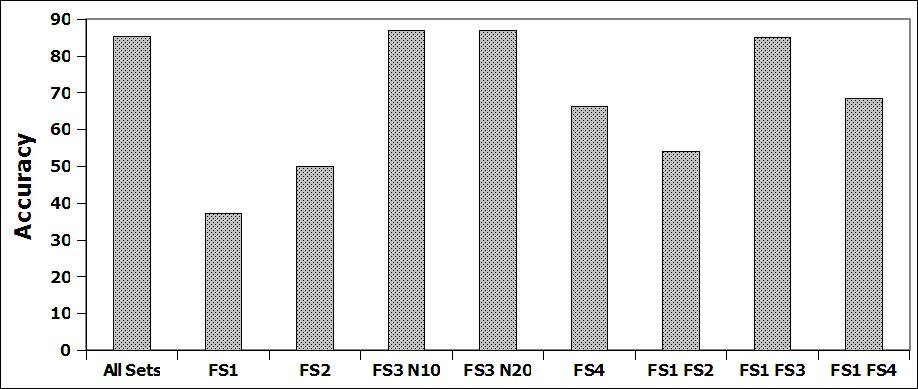
\includegraphics[scale=0.5]{images/featuresdifference.jpg}
	\caption{Feature Comparison on Hs-DB accuracy} The effect of different features on accuracy.  %The graph shows the recognition rate of each symbol using different algorithms. 
	\label{fig:testFeaturesAll}
\end{figure*}  


 \begin{figure*}
	\centering
		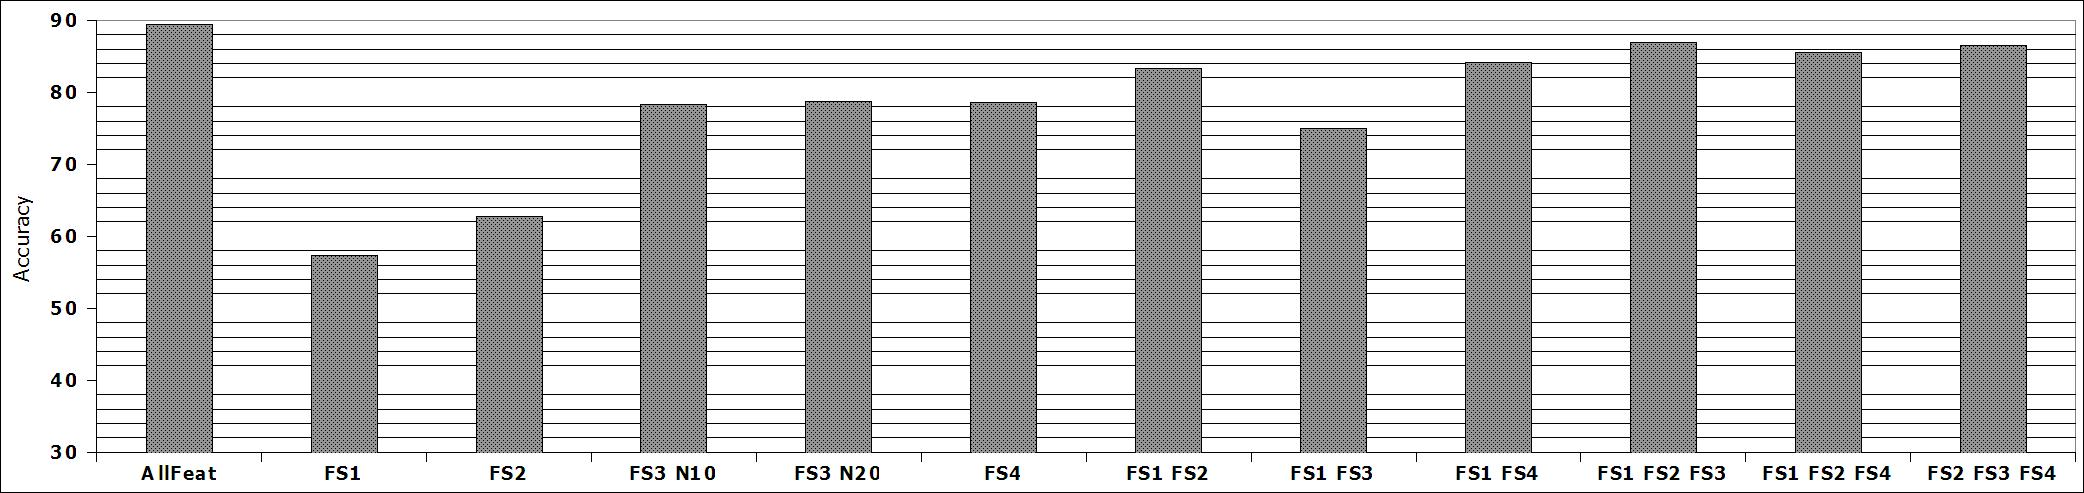
\includegraphics[scale=0.34]{images/featELc.jpg}
	\caption{Feature Comparison on EL-DB} The effect of different features on accuracy.  %The graph shows the recognition rate of each symbol using different algorithms. 
	\label{fig:ELtestFeaturesAll}
\end{figure*}  
 We could not test the result of the segmentation algorithm directly due to the fact that the correct segmentation is highly ambiguous. It is only based on what the user intends to draw while sketching the symbol. 
 The main features affected by the segmentation stage are the geometric features computed in \textbf{FS1}. Hence those are the features we used to estimate the efficiency of the segmentation algorithm. The recognition accuracy using only the geometrical features is reported in Figure \ref{fig:testFeatonly} . The figure shows that \textsl{AlgS2} achieve better results.  %effect of the segmentation algorithm 
 %Figure \ref{fig:SampleSeg} shows a sample of the output of the segmentation block. The result of segmentation block is tested by their effect on the final recognition results using the features that will be highly affected using different algorithms like \textbf{FS1} and \textbf{FS4} (Section\ref{sec:Recognition}). Figure \ref{fig:testFeatonly} shows the result of the different algorithms using only \textbf{FS1 }features. 
\begin{figure}
	\centering
		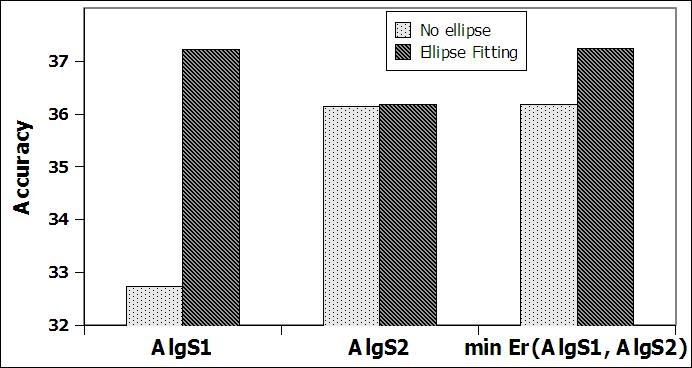
\includegraphics[scale=0.4]{images/featureFS1only.jpg}
	\caption{The effect of segmentation on Hs-DB accuracy} %The effect of symbol complexity.  %The graph shows the recognition rate of each symbol using different algorithms. 
	\label{fig:testFeatonly}
\end{figure}  

\begin{figure}[]
	\centering
				\subfigure[User strokes] {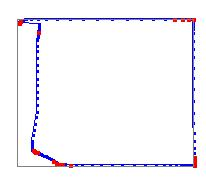
\includegraphics[scale=0.7]{images/strokebefore.jpg}}
		 	\subfigure[Segmented strokes] {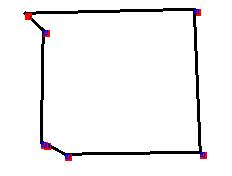
\includegraphics[scale=0.7]{images/strokeafter.jpg}}
		 		\subfigure[Multiple symbols] {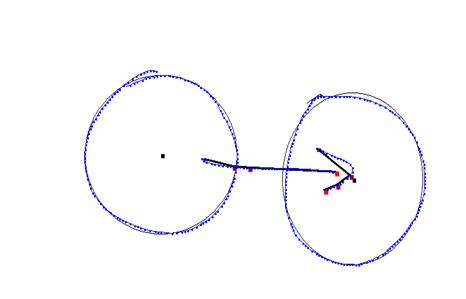
\includegraphics[scale=0.7]{images/results3.jpg}}
		
	\caption{Segmentation outputs}  The output segmentation of different input strokes. %The figure shows sample of the output of the segmentation phase. Figure a) shows the stroke after the user draws it. The red points are points labeled as \textit{possible dominate points}. Figure b) shows the symbol after being segmented. Figure c) shows the segmentation of different and overlapped strokes. Notice the system mark the center of the ellipse that was identified.
	\label{fig:SampleSeg}
\end{figure}

\section{Conclusion and Future Work}
\label{ConclusionandFutureWork}
This paper presented a new approach to sketch recognition using PSO. The system uses both speed and curvature information which help improving the \textit{DPSO}. It is noted that the \textit{DPSO} in general generates an optimized stroke segmentation which improves the final recognition rate.  The tradeoff between accuracy achieved and time complexity must be further investigated to achieve better results. The final recognition is based on both global shape and hierarchical stroke properties. Adding stroke and segment geometrical features improved the final recognition. Global shape and moment properties was used to prevent the need to use graph matching which is computationally expensive. The system was tested on 13 different symbols and achieved an overall accuracy of 89.5\%. The system does not depend on low level recognizer but rather on a set of high level features. This makes the system easily expandable to more and more symbols. 

 A possible extension of this research is to complete the clustering algorithm for fully automated sketch recognition. Currently, the system processes one symbol at a time, an enhancement would be to allow users to draw more than one symbol at a time and incorporate a method for separating symbols. Another area of enhancements is the features extraction methods. Introducing more spatial and geometrical features is believed to improve classifications. Features that represents the appearance of the symbols are likely to improve the recognition that have similar geometrical structure (i.e. Nand and And gate in logic symbols).  
 \bibliographystyle{elsarticle-harv} 
%\bibliographystyle{IEEEbib}
\bibliography{../../neededfiles/Bibliographies/Mybibliography}
\end{document}
